\documentclass[12pt,a4paper]{article}
\usepackage[utf8]{inputenc}
\usepackage[T1]{fontenc}
\usepackage{amsmath,amssymb,amsfonts}
\usepackage{hyperref}
\usepackage{geometry}
\usepackage{booktabs}
\usepackage{longtable}
\usepackage{amsthm}
\usepackage{graphicx}
\usepackage{tikz}
\usetikzlibrary{arrows.meta,positioning}
\newtheorem{theorem}{Theorem}
\newtheorem{proposition}[theorem]{Proposition}
\newtheorem{lemma}[theorem]{Lemma}
\newtheorem{corollary}[theorem]{Corollary}
\newtheorem{conjecture}[theorem]{Conjecture}
\theoremstyle{remark}
\newtheorem{remark}[theorem]{Remark}
\geometry{a4paper, margin=1in}
% ПРИ МЕЖДУНАРОДНОМ СЛИЯНИИ: замените титул на \part{I. Computational Mapping of the Collatz Space}
\title{The Architecture of the Collatz Space:\\Computational Mapping and Large-Deviation Theory}
\author{Collatz Crystal Hunter Project \\[0.5em] \small with AI Assistance}
\date{August 2026}
\begin{document}
\maketitle
\begin{abstract}
We present the results of a large-scale computational study of Collatz sequence
trajectories in terms of accelerated dynamics over odd numbers, shift-vectors,
and confluence structures. The central discovery is \textbf{Zone 2} --- a family
of 913 numbers with bit lengths 71--87, whose trajectories merge into a single
75-bit node $x^* = 20152090995747160937051$ in no more than 7 odd steps, after
which they follow an identical path to a peak of 140 bits. In parallel, Barina's
number was discovered --- a completely isolated second path to the same peak 140,
sharing no intermediate points with \textbf{Zone 2}. A systematic census of
confluence centers (peaks 10--200) revealed confluence centers for 39 peaks (all
integer peaks from 14 to 51, plus peak 140), establishing a continuous
archipelago. We discovered the formula
$\mathrm{center\_bits} = 0.498258 \cdot \mathrm{peak} + 6.2928$ ($R^2 = 0.965$,
primary centers) and the modular filter $c \equiv 2 \pmod 3$. Cluster analysis
divided all centers into two classes: \textbf{Class A} ($121$, $x^*$ --- ``deep
funnels'' with $d_{peak} \gg 10$, $S/d \approx 1.33$, 100\% hit rate) and
\textbf{Class B} (all others --- ``shallow confluences'' with
$d_{peak} \approx 3\text{--}15$, $S/d \approx 1.0\text{--}1.2$, hit rate
72--92\%). In the 88--170 bit range, an extensive ``dead zone'' without
anomalies above \textbf{Family A} is confirmed. The body of results indicates
that the Collatz space contains a continuous archipelago of confluence
structures (\textbf{Class B}), above which rise rare ``deep funnels''
(\textbf{Class A}), organized around the irrationality $\log_2 3$.
\smallskip
\noindent\textit{Supplementary Material:} All computational data, the full Zone 2
catalog (913 entries), algorithmic pseudocodes, and detailed derivations are
available in the Supplementary Material.

\smallskip
\noindent\textbf{Theoretical framework (Part II):} We develop a unified large-deviation theory of the Collatz (Syracuse) space that
explains the dichotomy between \emph{typical decay} and \emph{rigid confluence
structures}, and we show that the two are two faces of a single rate function.
We establish a chain of five linked results.
\textbf{(F1/R1)} The forward shift-vector obeys a large-deviation principle with
the Cram\'er rate of the geometric$(2)$ law, and the tilted $3$-adic reverse
operator obeys a backward large-deviation principle whose normalized rate
function coincides with the forward Cram\'er rate (\emph{duality}), verified
numerically ($\sim 10^{-3}$, hypothesis $I_{\rm rev} \equiv I_2$).
\textbf{(S1)} The generic peak-path is a \emph{soliton}---a typical path of the
exponentially tilted measure---and the fraction of peak-paths passing through
any confluence center vanishes.
\textbf{(I1)} Confluence centers are the rigid points of the same tilted
ensemble: \emph{dressed vacua}, the $(1,1,2)$ $3$-adic fixed point
$\xi=-29/11$ dressed by a sparse gas of topological charges with $O(1)$ total
charge.
\textbf{(C1)} Each center sits at the log-midpoint
$\mathrm{bits}(c)=\tfrac12 P+O(1)$, a detailed balance between the forward gain
cone and the conditioned backward entropy cone.
\textbf{(M1)} Reverse synthesis of macro-centers is algorithmically closed: a
CRT dimensionality deficit $\Delta\ge2P$ makes constructive assembly a
measure-zero event, so the Scaling $\times10$ hypothesis passes from
constructibility to ontology.
The reverse calculation yields the geometric ratio
$\gamma_{\rm rev}\approx0.993$, but attaching it to the forward exceptional set
requires an additional reverse-chord encoding hypothesis.  Independently, a
finite-scale $2$-adic counting argument gives an unconditional local descent
bound, while iteration across scales requires an open restart/transport lemma.
These distinctions delimit the present programme: anomalous structures can be
studied quantitatively, but no unconditional global exceptional-set exponent is
claimed.
\end{abstract}

\newpage
\tableofcontents
\newpage

\part{The Computational Map}
\section*{Glossary and Constants}
\begin{itemize}
\item \textbf{Family A ($2^b - 1$)}: The base landscape. Ratios tend to $\log_2 3 \approx 1.585$.
\item \textbf{Confluence}: The gravitational capture of trajectories into nodes (centers).
\item \textbf{Class A (Deep funnels)}: 100\% Hit Rate. Centers $121$ (Peak 14) and $x^*$ (Peak 140).
\item \textbf{Class B (Shallow funnels)}: 72--93\% Hit Rate. Dense archipelago (Peaks 14--51).
\item \textbf{Center Bits Formula}: $\mathrm{center\_bits} = 0.498258 \cdot \mathrm{peak} + 6.2928$ $(R^2 = 0.965)$, primary centers; the refit over all 39 centers is $0.620145 \cdot \mathrm{peak} + 2.2850$ $(R^2=0.916)$.
\item \textbf{Scaling Hypothesis $\times 10$}: Class A centers follow a logarithmic scale ($14 \to 140 \to 1400$). Status: constructive routes closed (all three obstructions); existence remains an open question.
\item \textbf{Septembrino's Law}: Distribution of divisors $P(\mathrm{div} = 2^a) = 1/2^a$.
\end{itemize}

\section{Introduction and Chronology of the Study}
\subsection{The Collatz Problem}
For a natural number $n$, define $T(n) = n/2$ if $n$ is even, and $T(n) = (3n+1)/2$ if odd. The Collatz conjecture states that iterations of $T$ for any $n$ eventually reach 1. Despite its elementary formulation, the problem remains open; Paul Erd\H{o}s remarked that ``mathematics may not be ready for such problems.''
The quantitative measure of a number's ``anomaly'' is its ratio --- the ratio of the trajectory's peak bit length to the input bit length. For typical numbers, ratio $\approx 1.0$--$1.2$. Numbers of the form $2^b - 1$ (Family A) yield a ratio approaching $\log_2 3 \approx 1.585$. Anything significantly higher represents a structural anomaly.

\subsection{Starting Point: David Barina's Results}
David Barina performed an exhaustive search of all numbers up to $2^{71}$ and compiled a table of path records. In Barina's table, there are two 71-bit record holders: $n = 2358909599867980429759$ (ratio 1.97, peak 140) and $n = 1765856170146672440559$ (ratio 1.97, peak 140). These numbers became the starting point of the entire study.

\subsection{Phase 1: Collatz Crystal Hunter and Markov Chains (February 2026)}
The first task was a directed search for numbers with an anomalously high ratio in the 72--80 bit range. The Collatz Crystal Hunter (v5.3a) system was developed --- a distributed Python program with hybrid candidate generation: a Markov chain of order 5 trained on found numbers; a pool of prefixes from Barina's path records with adaptive weights; three-stage filtering (50 steps culling ratio $<1.03$; 200 steps; full simulation to 50,000 steps); 35 workers via multiprocessing. In 10+ hours on 35 cores, the best found ratio for 73--80 bits was 1.613.

\subsection{Phase 2: Statistical Analysis of 30 Million Numbers (Early March 2026)}
The system collected 30 million records for bit lengths 72--80. The analysis revealed: the ratio distribution has a sharp peak around 1.04--1.05 and a fast-decaying tail (power law $\alpha \approx 3.66$); the median ratio monotonically decreases with bit length; the 99th percentile drops from 1.1528 (72 bits) to 1.1250 (80 bits). But the main discovery: the maximum ratio for each bit length dropped almost linearly ($\approx 0.024$ per bit), and recalculating $\max\_ratio \times bits$ for all bit lengths 72--80 yielded the exact same number: exactly 140 --- a ``magnetic peak'' towards which the trajectories of many extreme numbers tend.

\subsection{Phase 3: From Statistics to Structure (March 2026)}
The discovery of the ``magnetic peak'' 140 required a structural approach: why exactly 140? Which numbers produce this peak? A second-generation toolkit was developed: a CRT constructor (\texttt{crt\_solver.py}), a shift-vector analyzer, reverse trees, and beam search over residue classes. By the end of March 2026, all results described below were obtained.

\section{Notation and Accelerated Dynamics}
We consider the accelerated Collatz trajectory over odd values:
\begin{equation}
x_{k+1} = \frac{3 \cdot x_k + 1}{2^{a_k}}
\end{equation}
where $a_k \ge 1$ is the 2-adic valuation of $3x_k + 1$. The sequence $a_0, a_1, \dots, a_{d-1}$ is the shift-vector; $d$ is the number of odd steps to the peak; $S_k = a_0 + \cdots + a_{k-1}$ is the accumulated shift. After $k$ steps:
\begin{equation}
x_k = \frac{3^k \cdot x_0 + c_k}{2^{S_k}}, \quad c_0 = 0, \quad c_{k+1} = 3 \cdot c_k + 2^{S_k}.
\end{equation}
The cumulative gain is $G(k) = k \cdot \log_2 3 - S_k$. The peak is reached near the maximum of $G(k)$. Every prefix of the shift-vector defines a unique residue class $x_0 \equiv r_k \pmod{2^{S_k}}$, allowing reconstruction from parity strings via CRT.

\subsection{2-adic Interpretation}
In $p$-adic terminology, every admissible shift-vector $w$ defines a 2-adic cylinder $C(w) = \rho(w) + 2^{S_d} \cdot \mathbb{Z}_2$ with Haar measure $2^{-S_d}$. \textbf{Zone 2} is a cylinder of anomalously small measure ($2^{-342}$ for a 71-bit input); the number 27 defines a cylinder of measure $2^{-70}$, and Barina's number a cylinder of measure $2^{-271}$. The archipelago of confluence centers is a finite set of exceptional cylinders in $\mathbb{Z}_2$, separated by vast regions where the measure of growing paths is exponentially small --- consistent with Tao's (2019) almost-all decay.
\smallskip
\noindent\textbf{Remark 2.1} (Septembrino's parameterization).
The formula $N = k \cdot 3^m - 1$ parameterizes the Haar measure in $\mathbb{Z}_2$. The observed periodicity of $v_2(N)$ follows from $3^n \pmod{2^p}$, placing it within classical $p$-adic dynamics.

\section{Base Layer: Family A}
Numbers $n = 2^b - 1$ form the base surface: shift-vector almost all ones (94--97\%), ratio $\to \log_2 3$, $S/d \approx 0.99$ --- the ``landscape level''. Full spectral analysis of $2^b - 1$ for $b = 71\text{--}310$ revealed 10 values with $S/d > 1.05$: $b=113\text{--}114$ (peak 183), $b=117\text{--}118$ (peak 190), $b=173\text{--}176$ (peak 280, resonance $3^{183}\approx2^{290}$), $b=301\text{--}304$ (peak 483, resonance $3^{306}\approx2^{485}$), $b=309\text{--}310$ (peak 494). Verification showed micro-plateaus exist exclusively for $2^b-1$ itself and do not form families --- unlike \textbf{Zone 2}.

\section{Zone 2: The Only Confirmed Major Confluence Class}
\subsection{Discovery}
Analysis of Barina's record holders (71--82 bits) revealed they all peak at exactly 140 bits with shift-vectors almost identical from the 8th position, indicating a common ``core''. \textbf{Zone 2} numbers were found for all bit lengths 71--87.

\subsection{Table of Zone 2 Representatives}
\begin{longtable}{lllll}
\toprule
\textbf{Bits} & \textbf{Number $n$} & \textbf{Peak} & \textbf{Ratio} & \textbf{Steps to $x^*$} \\
\midrule
71 & 2358909599867980429759 & 140 & 1.9718 & 7 \\
72 & 4717819199735960859519 & 140 & 1.9444 & 7 \\
73 & 9435638399471921719037 & 140 & 1.9178 & 7 \\
74 & 18871276798943843438074 & 140 & 1.8919 & 7 \\
75 & 37742553597887686876149 & 140 & 1.8667 & 7 \\
76 & 75485107195775373752296 & 140 & 1.8421 & 7 \\
77 & 150970214391550747504611 & 140 & 1.8182 & 7 \\
78 & 301940428783101495009251 & 140 & 1.7949 & 7 \\
79 & 603880857566202990018507 & 140 & 1.7722 & 7 \\
80 & 1207761715132405980037043 & 140 & 1.7500 & 7 \\
81 & 2415523430264811960074099 & 140 & 1.7284 & 7 \\
82 & 4831046860529623920148297 & 140 & 1.7073 & 7 \\
83 & 9662093721059247840295139 & 140 & 1.6867 & 7 \\
84 & 19324187442118495680593175 & 140 & 1.6667 & 7 \\
85 & 38648379884236991361186739 & 140 & 1.6471 & 7 \\
86 & 77296749768473982722370787 & 140 & 1.6279 & 7 \\
87 & 154593499536947965444748439 & 140 & 1.6092 & 7 \\
\bottomrule
\caption*{One representative per bit length (of 913 known). All have $d=259$ odd steps to the peak and $S = \mathrm{bits}+271$.}
\end{longtable}

$2^{88}-1$ peaks at $141$ and does \emph{not} pass through $x^*$ --- the sharp boundary.

\begin{figure}[h]
    \centering
    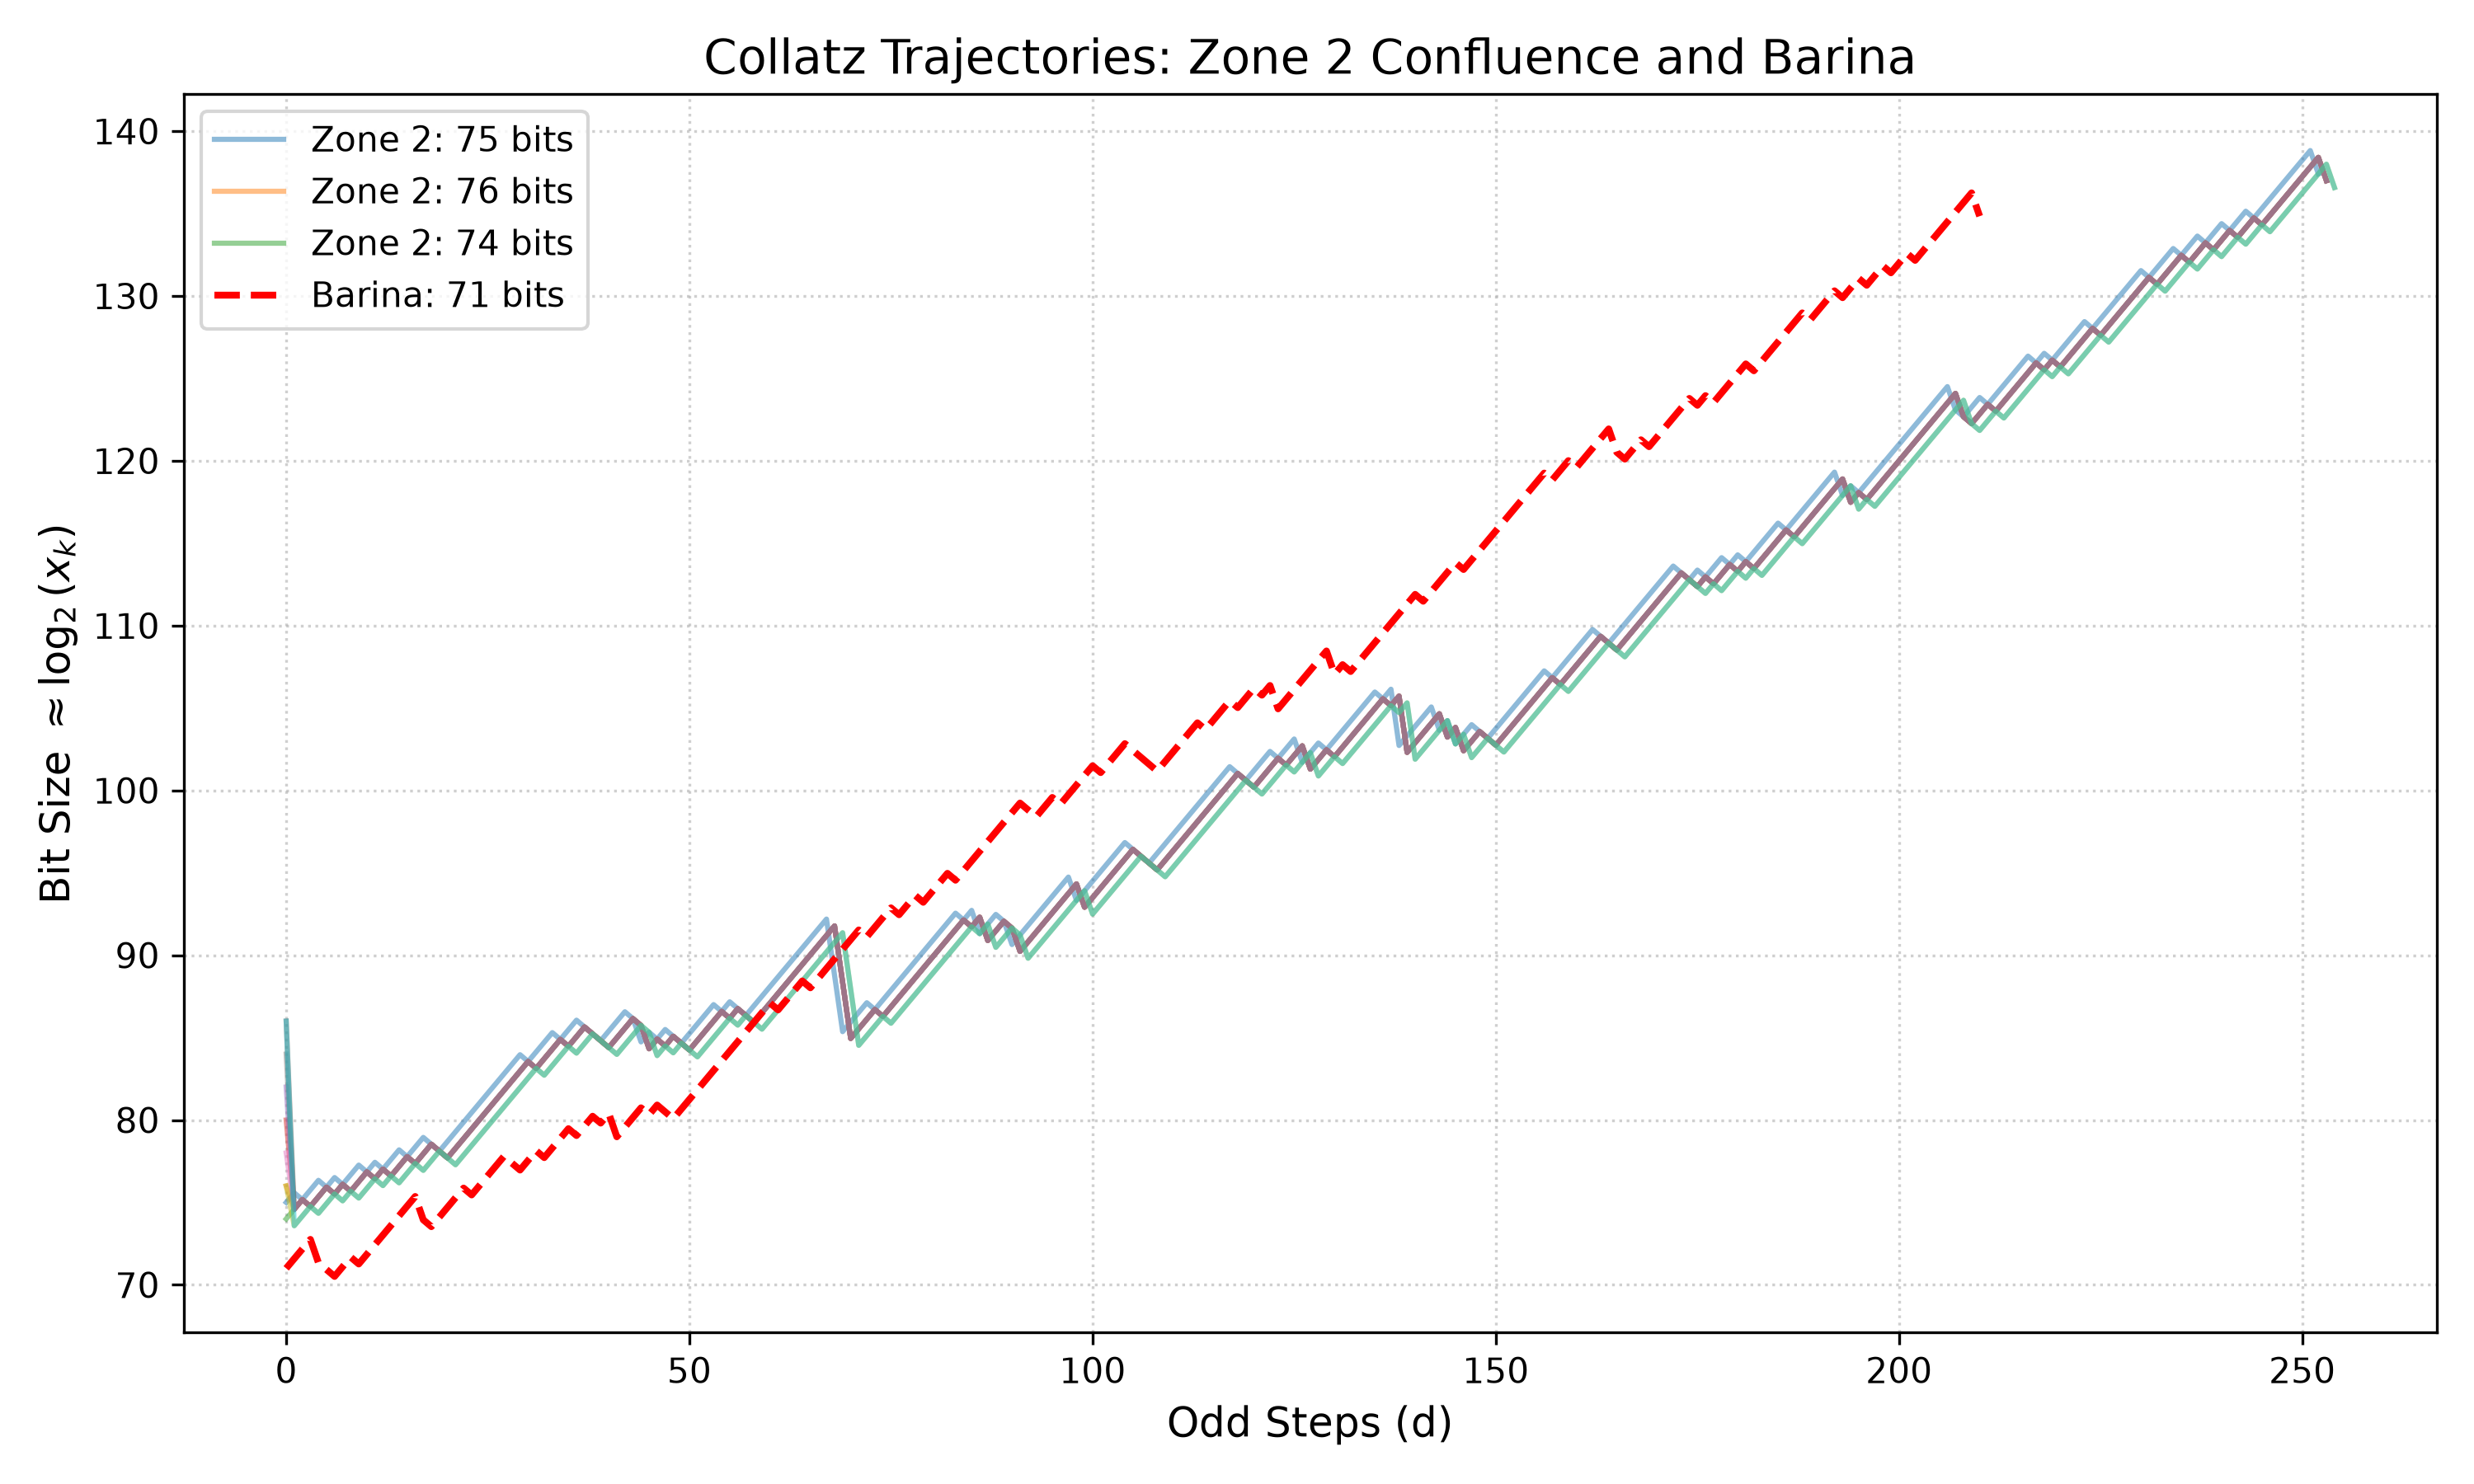
\includegraphics[width=0.8\textwidth]{../data/trajectory_plot.png}
    \caption{Trajectories of Zone 2 numbers (solid) perfectly merging into $x^*$, compared to Barina's number (dashed) reaching the same peak independently.}
    \label{fig:trajectory}
\end{figure}

\begin{figure}[ht]
\centering
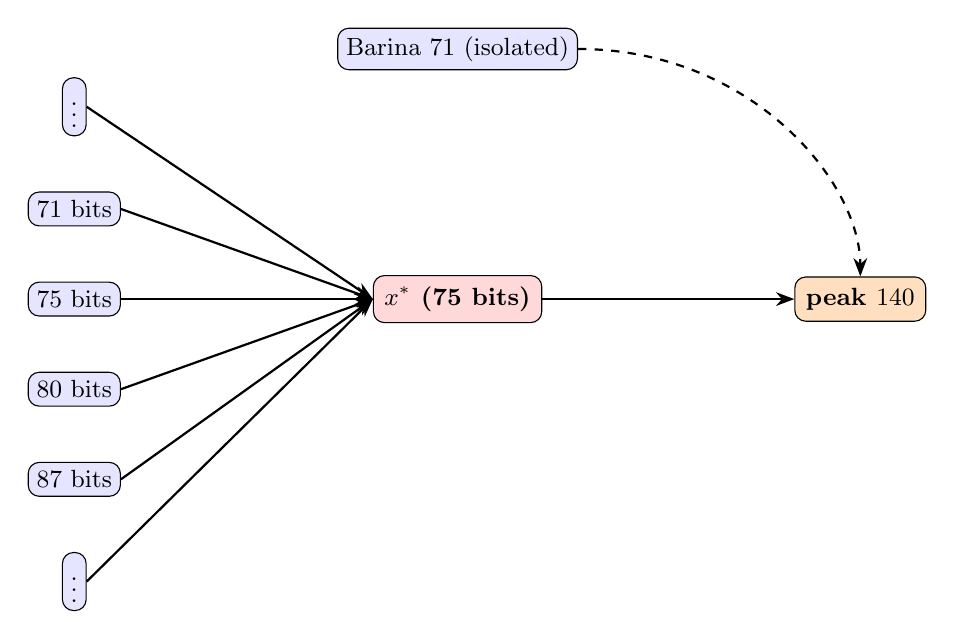
\begin{tikzpicture}[
  node distance=7mm and 20mm,
  innode/.style={draw,rounded corners,fill=blue!10,inner sep=3pt,font=\small},
  corenode/.style={draw,rounded corners,fill=red!15,inner sep=4pt,font=\small\bfseries},
  peaknode/.style={draw,rounded corners,fill=orange!25,inner sep=4pt,font=\small\bfseries},
  arr/.style={-{Stealth},thick}, darr/.style={-{Stealth},thick,dashed}]
\node[innode] (d0) {$\vdots$};
\node[innode,below=of d0] (i71) {$71$ bits};
\node[innode,below=of i71] (i75) {$75$ bits};
\node[innode,below=of i75] (i80) {$80$ bits};
\node[innode,below=of i80] (i87) {$87$ bits};
\node[innode,below=of i87] (d1) {$\vdots$};
\node[corenode,right=3.2cm of i75] (xs) {$x^*$ (75 bits)};
\node[peaknode,right=3.2cm of xs] (pk) {peak $140$};
\node[innode,above=2.6cm of xs] (bar) {Barina $71$ (isolated)};
\foreach \n in {d0,i71,i75,i80,i87,d1} {\draw[arr] (\n.east) -- (xs.west);}
\draw[arr] (xs) -- (pk);
\draw[darr] (bar.east) .. controls +(2.2,0) and +(0,1.2) .. (pk.north);
\end{tikzpicture}
\caption{Schematic reverse tree: 913 inputs (bits 71--87) collapse into $x^*$; Barina's number reaches the same peak by a disjoint path.}
\label{fig:confluence}
\end{figure}

\subsection{Two-Layer Invariants: Core and Adapter Shell}
A complete census of all 913 inputs reveals a two-layer structure.
\textbf{1. The Core ($x^* \to$ Peak).} All 913 numbers pass through $x^*$; the trajectory from $x^*$ to the peak is strictly identical, of length $d_{core} = 251$ odd steps and cumulative shift $S_{core} = 334$. The ratio $S_{core}/d_{core} \approx 1.331$ is the true constant of the basin.
\textbf{2. The Adapter Shell.} Numbers reach $x^*$ in $k \in [0,7]$ odd steps; 378 of 913 lie at maximum depth $k=7$, with total $d = 258$. An affine bit-burning law governs the outer shell: $S_{adapter} = \mathrm{bits} - 63$, so $S = \mathrm{bits}+271$ holds \emph{only} for the outer shell. Pre-image automata analysis yields a growth rate $\approx 0.395$ bits$^{-1}$ (close to the adapter topological entropy):
\begin{table}[h]
\centering
\begin{tabular}{llll}
\toprule
\textbf{Bits} & \textbf{Model Forecast ($0.395$ bit$^{-1}$)} & \textbf{Actual Reverse Tree} & \textbf{Error} \\
\midrule
88 & 287 & 272 & +5\% \\
89 & 379 & 331 & +15\% \\
90 & 497 & 343 & +45\% \\
\bottomrule
\end{tabular}
\caption{Retrospective forecast, accurate to 88 bits before finite-depth saturation.}
\end{table}
The adapter sequence is completely determined by the lowest 19 bits. \textbf{Zone 2} is an exact $d=251$ core path dressed in a deterministic pre-image tree.

\subsection{Confluence Point $x^*$}
\begin{theorem}[Computational]
All 17 representatives of \textbf{Zone 2} (bits 71--87, $d=259$) arrive, after $\le7$ odd steps, at the exact same number
$x^* = 20152090995747160937051$ (75 bits). After this point the trajectories are literally identical for 252 steps until the peak of 140. $2^{88}-1$ does not pass through $x^*$.
\end{theorem}

\subsection{Reverse Tree of $x^*$ and Full Size of Zone 2}
The reverse tree of predecessors of $x^*$ to depth 7 (bits $\le 90$) revealed 1859 nodes, of which 913 have bits 71--87; every one yields peak 140 (100\%):
\begin{longtable}{llll}
\toprule
\textbf{Bits} & \textbf{Nodes in Tree} & \textbf{With Peak 140} & \textbf{Fraction} \\
\midrule
71 & 1 & 1 & 100\% \\ 72 & 2 & 2 & 100\% \\ 73 & 4 & 4 & 100\% \\
74 & 7 & 7 & 100\% \\ 75 & 7 & 7 & 100\% \\ 76 & 8 & 8 & 100\% \\
77 & 9 & 9 & 100\% \\ 78 & 14 & 14 & 100\% \\ 79 & 20 & 20 & 100\% \\
80 & 33 & 33 & 100\% \\ 81 & 47 & 47 & 100\% \\ 82 & 62 & 62 & 100\% \\
83 & 78 & 78 & 100\% \\ 84 & 100 & 100 & 100\% \\ 85 & 129 & 129 & 100\% \\
86 & 173 & 173 & 100\% \\ 87 & 219 & 219 & 100\% \\
\midrule
\textbf{Total} & \textbf{913} & \textbf{913} & \textbf{100\%} \\
\bottomrule
\end{longtable}
The number of inputs approximately doubles with each bit.

\subsection{Grammar of the Shift-Vector}
Spectral analysis (FFT) of all 913 vectors shows pronounced peaks at periods $T \approx 10$, $6.3$, $18$. In the critical tail, a staircase $[2,1,1]$ frequently emerges --- the shadow of the 3-adic periodic point $-29/11$ (fixed point of inverse $(1,1,2)$ steps), linking the deterministic core with the control-budget limitations.

\subsection{The $(1,1,2)$ Equilibrium and the Attractor $4/3$}
\begin{lemma}[$(1,1,2)$ periodic equilibrium]
Consider the reverse map $R_a(x)=(x\cdot 2^{a}-1)/3$. The composition over one period $(1,1,2)$ is $F(x)=\frac{16x-29}{27}$, a contraction on $\mathbb{Z}_2$ ($|16/27|_2=2^{-4}<1$) with unique fixed point $\xi=-29/11$. The periodic orbit of $\xi$ has mean shift $4/3$ and gain rate $\log_2 3-4/3\approx0.2516$ bits/step, matching the observed body growth $\sim0.25$.
\end{lemma}
\begin{theorem}[Core as dressed equilibrium; computational]
The \textbf{Zone 2} core satisfies $S_{core}/d_{core}\approx1.331$, within $0.2\%$ of $4/3$. Hence the core is the $(1,1,2)$ vacuum $\xi=-29/11$ dressed by a sparse gas of topological charges (defects $a\ge3$) shifting the mean by $<0.2\%$. (Rigorous formulation: Part~II, Theorem~I1.)
\end{theorem}
\paragraph{Connection to the Control Budget.}
The $4/3$ equilibrium sits below the critical limit $\bar a_p=\log_2 3\approx1.585$; any defect $a\ge3$ requires a compensating pure run $L \ge (a-\bar a_t)/(\bar a_t-\bar a_p)$. Since the vacuum leaves no free margin, macroscopic structural solitons cannot be constructed arbitrarily.

\section{Barina's Number: An Isolated Second Path to Peak 140}
Barina's number $n = 1765856170146672440559$ (71 bits, $d=213$, $S/d=1.263$) reaches peak 140 via a completely different path.
\begin{lemma}[Barina's isolation]
Between the trajectories of Barina's number and any \textbf{Zone 2} number ($d=259$) there is not a single common intermediate point --- even modulo $2^{30}$. The common prefix is the trivial $[1,1,1]$; the common suffix is empty. The reverse tree from Barina's peak is empty (its peak odd value $\equiv0\pmod3$ has no integer predecessors).
\end{lemma}
This is a counterexample to the naive idea that a high peak determines structure: the same peak 140 is achieved by at least two independent mechanisms.

\section{Number 27 as a Miniature Zone 2}
The trajectory of 27 has $d_{peak}=28$, $S/d\approx1.36$, shift-vector 58.5\% ones, 24.4\% twos, 7.3\% threes --- almost identical to \textbf{Zone 2}. The value $x_7=121$ is a confluence center: the reverse tree from 121 to depth 5 contains 27 numbers, all with peak 14 (100\%). Pre-image automata give similarity $\approx0.989$ between $x^*$ and $121$.
\begin{table}[h]
\centering
\begin{tabular}{lll}
\toprule
\textbf{Parameter} & \textbf{n = 27} & \textbf{Zone 2 (core)} \\
\midrule
Center & $121$ (7 bits) & $x^*$ (75 bits) \\
Peak & 14 & 140 \\
Inputs & 27 & 913 \\
$S/d_{to\_peak}$ & $\sim 1.36$ & $\sim 1.33$ \\
\% ones & 58.5\% & 74\% \\
Dips in $G(k)$ & 17 & 67 \\
\bottomrule
\end{tabular}
\end{table}

\section{Dead Zone 88--170 Bits}
In 88--170 bits, not a single number with ratio $>1.585$ was found, despite four independent methods:
\begin{enumerate}
\item Peak hunter + zone\_search (evolutionary, millions of candidates): zero anomalies.
\item Parity scan (\texttt{zone\_parity\_search.py}), $d=80$--$500$, CRT reconstruction, $>14$M checks: zero.
\item Beam search without niching (\texttt{residue\_search.py}), 3 filters, 150,000 verifications: zero for bits $>89$.
\item Beam search with niching (5 bins by $S/d$), 300,000 verifications: zero for bits $>93$.
\end{enumerate}
\begin{corollary}
After \textbf{Zone 2} (boundary 87 bits), the Collatz space shows no new confluence \emph{ratio} anomalies up to 170 bits.
\end{corollary}

\subsection{Probabilistic Anatomy of the Dead Zone}
Under the i.i.d.\ shift heuristic, Sanov's theorem gives the probability of a vector with $S/d\le1.40$ falling as $2^{-d\cdot0.28}$, where $0.28\approx D_{\mathrm{KL}}(q\|p)$ between the Zone-2 profile $q\approx(0.75,0.21,0.04)$ and $p(a)=2^{-a}$. For $d>300$ this is $<10^{-25}$. (Shifts are correlated, so this is a strong heuristic, not a strict bound.)

\subsection{The Algebraic Impossibility of Shadow Zones}
A constructive ``shadow'' scenario (cloning a known anomalous block $w$) is obstructed by a CRT dimensionality effect.
\begin{proposition}[CRT dimensionality trap]
Let $w$ be admissible with total shift $S$, and $m\ge1$. The exact $m$-fold self-similar extension $w^m$ occupies a single residue class modulo $2^{mS}$. If $B<mS$, the number of $B$-bit integers realizing it is at most one, with expected count $\mathbb E N(B;w,m)\approx2^{B-mS}$.
\end{proposition}
\begin{proof}
$w^m$ has total shift $mS$, defining one cylinder mod $2^{mS}$; the $B$-bit interval has length $\approx2^B<mS$, so a fixed residue class meets it in $\le1$ point; Haar expectation $\approx2^B2^{-mS}$.
\end{proof}
For Barina ($S\approx269$) a two-fold echo at $B=142$ has expectation $2^{-396}$; for Zone~2 ($S=342$--$358$) $\le2^{-514}$; for $x^*$ ($S\approx334$) $\le2^{-496}$.
\begin{table}[h]
\centering
\caption{CRT dimensionality obstruction for exact two-fold echoes.}
\begin{tabular}{lccccc}
\toprule
\textbf{Known block} & $d$ & $S$ & \textbf{Modulus (2 copies)} & \textbf{Target} $B$ & \textbf{Expected count} \\
\midrule
Barina & 213 & $\approx269$ & $2^{538}$ & 142 & $2^{-396}$ \\
Barina & 213 & $\approx269$ & $2^{538}$ & 170 & $2^{-368}$ \\
Zone~2 core & 259 & $342\text{--}358$ & $2^{684}\text{--}2^{716}$ & $\le170$ & $\le2^{-514}$ \\
$x^*$ core & 251 & $\approx334$ & $\approx2^{668}$ & $\le170$ & $\le2^{-498}$ \\
\bottomrule
\end{tabular}
\end{table}
Thus the dead zone is protected by two mechanisms: \emph{entropic} (Sanov) and \emph{algebraic} (CRT dimensionality). A miraculous one-off solution cannot be excluded by measure alone; to exclude it for a chosen $B$ one must compute the exact CRT lift and check it lies in $[2^{B-1},2^B)$.
\paragraph{Experimental confirmation (CRT Lift).} Direct lifts found exact two-fold echoes: Zone~2 core at $x_0\approx2^{670}$ (peak 799, ratio $1.1925$); Barina at $x_0\approx2^{544}$ (peak 682, ratio $1.2537$) --- confirming constructive access near $B\approx2S$, but with ratios strictly below the Family~A boundary $1.585$: high-ratio anomalies remain unconstructable.

\subsection{The Control-Budget Obstruction to Constructive Macro-Solitons}
\begin{lemma}[Defect compensation]
Since the defect-free $(1,1,2)$ equilibrium has mean $\bar a_p\in[1.33,4/3]$, a defect $a\ge3$ forces a clean run $L\ge(a-\bar a_t)/(\bar a_t-\bar a_p)$. For $\bar a_t=1.35$, $a=3$: $L\in[82.5,99]$.
\end{lemma}
\begin{lemma}[Measure of clean runs]
A child admits a clean run of length $L$ with expected fraction $(2/3)^L$ (stepwise-independence heuristic, validated by mod-3 balance $50/50$, killer fraction $1/3$).
\end{lemma}
\begin{theorem}[Control budget]
A policy with branching $B$ per defect survives only if $B(2/3)^L\ge1$, i.e.\ $L\le\ln B/\ln(3/2)$. For $B=4$, $L_{\max}\approx3.4\ll L_{\min}\approx82.5$--$99$. Required $B\sim10^{14}$--$10^{17}$ is scale-independent.
\end{theorem}
\begin{corollary}[Closure of constructive Scaling $\times10$]
No bounded-branching constructive lifting assembles a Class~A macro-soliton; $14\to140\to1400$ is closed for constructive methods.
\end{corollary}
\begin{remark}[Existence vs.\ constructibility]
The obstruction is algorithmic, not ontological. Zone~2 itself is not constructible (margin $\bar a_t-\bar a_p\approx10^{-3}$, $L_{\min}(3)\approx1666$); it was found by reverse enumeration \emph{from an aligned node}. Solitons can be found, not grown.
\end{remark}
\paragraph{Experimental confirmation.} Runs with increasing control authority (plain corridor; mod-9 steer; 6-adic lookahead) died at steps $261,173,136$ --- monotone worsening, as predicted. At macro scale (peak 1400) the beam died at step 24, because a length-6 macro-block applies only from a specific class mod $729$ and the 93-block grammar covers $12.7\%$ of states: the instanton grammar is a coordinate chart of one rigid object, not a generative grammar.

\section{Refutation of Zone 3}
Candidates with peaks 237--244 (145--150 bits) are the neighborhood of \textbf{Family A}: the core of 112 single shifts follows from $\sim100\%$ ones density; peak $\approx$ bits $+65.5+L\cdot1.585-tail$; bit-inversion fragility identical to Family~A; independent generation showed all such numbers were $2^b-1$ themselves. Zone 3 does not exist.

\section{Archipelago of Confluence Centers}
\subsection{Systematic Census (Peaks 10--200)}
A systematic census expanded an initial 5 centers; reverse-tree verification confirmed 12 for peaks 14--30; directed search with algebraic filters discovered centers for \emph{every} peak 31--50 (up to $5.7\times10^9$ candidates/peak). The census also identified recurring descent transit hubs (2051, 23) --- infrastructure, not caustics; confluence mapping must filter out descent coincidences.
\begin{longtable}{lllllll}
\toprule
\textbf{Peak} & \textbf{Center} & \textbf{Bits} & \textbf{Inputs} & \textbf{Hit rate} & $d_{peak}$ & $S/d$ \\
\midrule
14 & 719 & 10 & 33 & 80.5\% & 3 & 1.00 \\
14 & $121$ (\textbf{A}) & 7 & 27 & 100\% & 21 & 1.38 \\
15 & 1127 & 11 & --- & 75.0\% & --- & --- \\
16 & 6803 & 13 & 22 & 84.6\% & 1 & 1.00 \\
17 & 3503 & 12 & --- & 87.5\% & --- & --- \\
18 & 27611 & 15 & 25 & 86.2\% & 4 & 1.25 \\
19 & 15977 & 14 & 39 & 72.2\% & 9 & 1.33 \\
20 & 4763 & 13 & --- & 100\% & --- & --- \\
21 & 52487 & 16 & 37 & 77.1\% & 11 & 1.36 \\
22 & 61823 & 16 & 55 & 74.3\% & 6 & 1.00 \\
23 & 41471 & 16 & 104 & 82.5\% & 15 & 1.20 \\
24 & 586115 & 20 & 32 & 82.1\% & 22 & 1.50 \\
25 & 705307 & 20 & 28 & 77.8\% & 8 & 1.13 \\
26 & 1085723 & 21 & 52 & 75.4\% & 7 & 1.14 \\
27 & 4918427 & 23 & 36 & 81.8\% & 10 & 1.30 \\
28 & 124463 & 17 & --- & 100\% & --- & --- \\
29 & 195923 & 18 & --- & 100\% & --- & --- \\
30 & 58595471 & 26 & 31 & 81.6\% & 3 & 1.00 \\
31 & 48427561 & 26 & 20 & 83.3\% & 10 & 1.30 \\
32 & 1242665 & 21 & 165 & 85.1\% & 27 & 1.26 \\
33 & 3538943 & 22 & 126 & 82.9\% & 16 & 1.00 \\
34 & 4205807 & 23 & 174 & 88.3\% & 28 & 1.25 \\
35 & 26658983 & 25 & 115 & 79.9\% & 61 & 1.46 \\
36 & 8524379 & 24 & 224 & 91.1\% & 53 & 1.38 \\
37 & 67625867 & 27 & 138 & 87.3\% & 69 & 1.46 \\
38 & 16348007 & 24 & 278 & 91.1\% & 36 & 1.28 \\
39 & 19351295 & 25 & 332 & 89.5\% & 39 & 1.28 \\
40 & 35337455 & 26 & 343 & 91.7\% & 41 & 1.27 \\
41 & 37748015 & 26 & 418 & 92.3\% & 81 & 1.42 \\
42 & 72481007 & 27 & 427 & 91.6\% & 64 & 1.38 \\
43 & 467269499 & 29 & 278 & 80.6\% & 38 & 1.26 \\
44 & 108893737 & 27 & 454 & 86.1\% & 51 & 1.29 \\
45 & 236651489 & 28 & 483 & 83.9\% & 62 & 1.35 \\
46 & 516844415 & 29 & 520 & 92.9\% & 50 & 1.28 \\
47 & 442441855 & 29 & 548 & 87.1\% & 54 & 1.30 \\
48 & 2303929595 & 32 & 520 & 92.9\% & 111 & 1.45 \\
49 & 3830005073 & 32 & 520 & 83.3\% & 73 & 1.38 \\
50 & 1396693151 & 31 & 716 & 88.5\% & 53 & 1.26 \\
51 & 6572463707 & 33 & $\approx400$ & 88.0\% & 56 & 1.29 \\
140 & $x^*$ (\textbf{A}) & 75 & 913 & 100\% & 250 & 1.33 \\
\bottomrule
\caption*{Confirmed confluence centers.}
\end{longtable}
The algebraic anatomy revealed: Law 1, $\mathrm{center\_bits}=0.498258\,\mathrm{peak}+6.2928$ ($R^2=0.965$); Law 2, $c\equiv2\pmod3$ (92\%); Law 3, $v_2(3c+1)=1$ (87\%).

\subsection{Two Classes of Centers}
Hierarchical clustering stably separates $\{121\}$ and $\{x^*\}$ (Class~A) from the Class~B mass.
\begin{table}[h]
\centering
\begin{tabular}{lll}
\toprule
\textbf{Metric} & \textbf{Class A ($121$, $x^*$)} & \textbf{Class B} \\
\midrule
Hit rate & 100\% & 72--92\% \\
$S/d$ to peak & 1.357 & 1.252 \\
bits/peak & 0.518 & 0.729 \\
$d_{peak}$ & 135.5 & 27.7 \\
Shift-profile & 70\% ones, 25\% twos & 80\% ones, 16\% twos \\
\bottomrule
\end{tabular}
\end{table}
Class~A centers are ``early gates'' through which all trajectories with a given peak must pass; their shift-profile is practically identical to the Zone~2 core.

\subsection{Trends and Transitional Centers}
Hit rate grows with peak ($+0.0036$/peak, $R^2=0.45$); inputs grow with peak; $S/d$ stable ($\approx1.27$). Five centers (peaks 35, 37, 41, 48, 49) occupy an intermediate position ($S/d>1.40$, $d_{peak}>50$) but hit rate $<100\%$.
\begin{remark}[Continuum of caustics]
Depth-resolved hit rate shows genuine ascending centers reach $HR=1.0$ as the window deepens (local caustics identical in kind to Class~A), while descending transit hubs dissolve ($HR\to0$). Class~A and Class~B form a continuum of caustics parameterized by compactness; Class~A is the extreme compact end.
\end{remark}
\subsection{Depth-Resolved Hit Rate: Class A as a Singular Class}
At fixed reserve $\Delta P\approx1$, Class~B and Transitional centers collapse to 46--78\% (or zero) by depth 4--5, while $x^*$ holds $\ge95.9\%$ to depth 9. Class~A is singular; the archipelago consists exclusively of Class~B funnels.
\subsection{Centers Do Not Cover the Space}
For 17,000 random numbers: 156 (0.92\%) pass through a center; among ratio $>1.5$: 0/14. Centers explain specific families, not the space as a whole.

\section{Spectrum of Chords: From Number 27 to Zone 2}
\begin{table}[h]
\centering
\begin{tabular}{lllll}
\toprule
\textbf{Type} & $S/d$ & \textbf{\% ones} & \textbf{Dips} & \textbf{Examples} \\
\midrule
\textbf{Family A} & 0.99 & 95--97\% & 3--7 & $2^{83}-1$ \\
Weak chord & 1.05 & 94\% & 5--8 & $2^{117}-1$ \\
Intermediate & 1.19 & 87\% & 22 & $2^{113}-1$ \\
\textbf{Zone 2} (Barina) & 1.26 & 78\% & 47 & 71 bits \\
\textbf{Zone 2} (core) & 1.32 & 74\% & 67 & 71--87 bits \\
Number 27 & 1.36 & 67\% & 11 & 5 bits \\
\bottomrule
\end{tabular}
\end{table}
$S/d$ is the ``chord strength'': a continuous spectrum in which Zone~2 and 27 occupy the same range.

\section{Summary Map of the Collatz Space}
{\small\sloppy
\begin{longtable}{p{2.5cm}p{1.4cm}p{0.7cm}p{0.9cm}p{0.7cm}p{2.0cm}p{2.2cm}}
\toprule
\textbf{Type} & \textbf{Bits} & \textbf{Pk} & $d$ & $S/d$ & \textbf{Class} & \textbf{Status} \\
\midrule
121 (confluence) & 5--13 & 14 & 21 & 1.38 & A & CONFIRMED \\
Continuous arch. & varies & 14--51 & 1--81 & 1.0--1.5 & B & 39 centers \\
Center formula & --- & --- & --- & --- & --- & $\mathrm{bits}\approx\mathrm{peak}/2+6.5$ \\
\textbf{Zone 2} & 71--87 & 140 & 259 & 1.33 & --- & 913 inputs \\
$x^*$ & $\sim38$ & 140 & 251 & 1.33 & A & CONFIRMED \\
Barina & 71 & 140 & 213 & 1.26 & --- & ISOLATED \\
Dead zone & 88--170 & --- & --- & --- & --- & 4 methods, 0 anom. \\
Plateau 280/483 & 173--176 / 301--304 & 280/483 & --- & $\sim1.0$ & --- & Resonance \\
Macro-centers & varies & $>50$ & varies & varies & --- & $\Delta\ge2P$, non-constructible \\
\bottomrule
\end{longtable}
}
The ``dead zone'' refers to the absence of ratio anomalies, not of confluence centers: Class~B centers exist for every peak but do not generate ratio anomalies.

\section{The Big Picture}
\begin{enumerate}
\item \textbf{Family A} --- base layer; plateaus 280/483 as $\log_2 3$ resonances.
\item Continuous archipelago of Class~B centers for all peaks 14--51.
\item Two Class~A deep funnels ($121$, $x^*$) --- early gates, Zone-2-like dynamics.
\item Crystals cannot be grown, only found (triad of obstructions).
\item Zone~2 --- unique large basin, most pronounced Class~A representative.
\item Barina's number --- independent isolated path.
\item Number 27 --- miniature Zone~2.
\item Dead zone 88--170 confirmed.
\end{enumerate}
The Collatz space is a continuous field of confluence structures (Class~B) above which rise rare deep funnels (Class~A).

\section{Computational Complexity}
Exhaustive parity scan $\mathcal O(2^{bits})$ (unfeasible $>90$); reverse tree $\mathcal O(B^{depth})$; residue beam search (exponential pruning, to 170 bits); confluence census ($22.9\times10^9$ candidates for peak 51, algebraic filter $\times3$ speedup).

\section{Open Questions}
Does the archipelago continue beyond peak 50? Does an aligned node $x^{**}$ exist for peak 1400 (existence, not constructibility)? Why $\alpha\approx1/2$? Through which point does Barina arrive? Connection to Tao's theorem and $\mathbb Z_2$-corridor stability of centers?

\appendix
\section{Main Project Scripts}
\textbf{Core:} \texttt{crt\_solver.py}, \texttt{records\_data.py}. \textbf{Search:} \texttt{peak\_hunter.py}, \texttt{zone\_parity\_search.py}, \texttt{residue\_search.py}, \texttt{class\_a\_search\_51\_80.py}. \textbf{Zone 2:} \texttt{confluence\_search.py}, \texttt{reverse\_tree\_xstar.py}, \texttt{count\_zone2\_in\_tree.py}, \texttt{analyze\_barina.py}. \textbf{Centers:} \texttt{confluence\_census.py}, \texttt{verify\_census\_centers.py}, \texttt{targeted\_search\_31\_50.py}, \texttt{targeted\_search\_41\_50.py}, \texttt{algebra\_centers.py}, \texttt{two\_class\_analysis.py}, \texttt{basin\_test.py}. \textbf{Spectrum:} \texttt{family\_a\_spectrum.py}, \texttt{check\_microplateau.py}, \texttt{analyze\_records\_gain.py}, \texttt{analyze\_27.py}. \textbf{Automata:} \texttt{automaton\_invariants.py}, \texttt{automaton\_compare.py}.

\subsection*{Key Algorithmic Primitives}
\begin{enumerate}
\item \textbf{Confluence filter:} $c\equiv1\pmod2$, $c\equiv2\pmod3$, $v_2(3c+1)=1$, $|\mathrm{bits}(c)-(0.498P+6.29)|\le3$ (rejects $\approx5/6$).
\item \textbf{Reverse step:} $T^{-1}(x,a)=\{(x2^a-1)/3\}$, $a=1..15$, odd positive only.
\item \textbf{Hit rate:} $HR(c,P;d_{win},W)=|\{y\in V_{d_{win}}\cap W:\mathrm{peak}(y)=P\}|/|V_{d_{win}}\cap W|$.
\item \textbf{Class A:} $HR=1.0$ for some window, $d_{peak}>20$, $S/d_{peak}>1.30$.
\end{enumerate}

\section{Nature of the Instanton (Expedition B)}
\begin{lemma}[2-adic vacuum]
$I=I_2\circ I_1\circ I_1$ is a contraction on $\mathbb Z_2$ (ratio $2^{-4}$) with unique fixed point $\xi=-29/11$, generating a periodic inverse orbit with $S/d=4/3$. Finite orbits shadowing $\xi$ to $2^{-m}$ over $d$ steps have $S/d=4/3+O(1/d)+O(2^{-m})$.
\end{lemma}
\begin{lemma}[Gain/charge balance]
For $w$ of length $d$, $S=\tfrac43 d+\delta$: $G(d)=d(\log_2 3-\tfrac43)-\delta$. Zone~2 core ($d=251$, $P-B\approx68.4$): $\delta\approx-0.67$ (low defect density).
\end{lemma}
\textbf{Hypothesis B3 (center as log-midpoint).} For Class~A centers, $\mathrm{bits}(c)\approx P/2+6.5$; the center is the deepest common node with sufficient cylinder measure. (Rigorous form: Part~II, Theorem~C1.)

\part{Large-Deviation Theory}


\section*{Data Availability and Formalization}
The full Zone 2 catalog (913 entries, \texttt{zone2\_shifts\_full.csv}), 39-center census, KL derivation, beam-search death logs, algorithmic pseudocodes, and Python verification scripts are available in the project GitHub repository. The Lean 4 formalization of the exact conditional transport (Theorem~\ref{thm:exact_conditional_transport}) and the CRT dimensionality obstruction (Theorem~M1) are also provided in the repository.

\begin{thebibliography}{99}

\end{thebibliography}
\end{document}
